% ~ 12 pages
\chapter{Identification of Hadronic Tau Lepton Decays using Boosted Decision
  Trees}
\label{sec:bdt}
The reconstruction of hadronic tau lepton decays described in
Chapter~\ref{sec:reconstruction} is based on the reconstruction of jets using
the anti-$k_\text{T}$ jet algorithm operating on clusters of calorimeter cells.
Jets originating from quarks or gluons, which are more abundant than tau leptons
due to the large multijet production cross section at the LHC, are often
reconstructed as candidates for hadronic tau lepton decays and represent a
significant background in many analyses. The reconstruction itself offers little
rejection of multijet events with the exception of the track classification
(cf.\ Section~\ref{sec:reco_track_sel_classif}) when requiring 1- or 3-prong
decays. In the ATLAS experiment an identification algorithm based on
multivariate methods utilising track and shower shape variables is used to
discriminate hadronic tau decays from multijet events.

This chapter will start with a description of the tau identification procedure
including definitions of the discriminating variables and the configuration of
the BDTs used for distinguishing hadronic tau decays (hereafter called signal)
and tau candidates from multijet events (hereafter called background). The
simulated samples used for training and performance evaluation of the models,
the kinematic reweighting and the preselection are described in
Section~\ref{sec:bdt_eventsim}. In Section~\ref{sec:bdt_hyperparam} a systematic
optimisation of the BDT configuration is performed to improve the overall
rejection of the identification. Subsequently, the variable selection is
investigated to improve the rejection by adding new variables and removing
variables only contributing little to the overall identification performance.
The chapter is concluded by evaluating the performance of the optimised BDTs.

In the following the signal efficiency, i.e.\ the fraction of reconstructed tau
candidates originating from hadronic tau decays passing a selection, will be
referred as the \emph{efficiency}. The \emph{rejection} refers to the inverse
background efficiency, i.e.\ the inverse fraction of tau candidates from
multijet events and pile-up passing a selection. The aim of this chapter is to
improve the rejection of multijet events at a fixed signal efficiency such that
analyses using tau identification observe larger signal-to-background ratios.

\todo[inline]{Working point efficiencies for pt and mu\\
  Rejection for full pt range;\\
  Plot 2nd order effects? (e.g.\ ptRatioEflowApprox vs.\ mEflowApprox 1p
  or massTrkSys vs.\ EMPOverTrkSysP 3p); \\
  Partial dependence plots; \\
  Understand the rejection vs.\ pt curve. Why does the rejection drop (is it
  because rejection is enhanced due to pile-up fakes)? Why does rejection
  increase again for high pt?; \\
  BDT is optimised for a 'gammatautau'-like spectrum (focused on improving
  rejection at low pt);}

\section{Description of the Tau-Identification Procedure}
\label{sec:bdt_tauid}
The tau identification algorithm currently in use in the ATLAS experiment
employs BDTs with high-level input variables. The identification uses separate
BDTs for 1- and 3-prong hadronic tau lepton decays with different sets of input
variables. Classification with BDTs return a score measuring the confidence of
the binary decision. This allows a trade off between signal efficiency and
background rejection by choosing different decision thresholds. In the ATLAS
experiment these thresholds are parametrised as functions of the reconstructed
visible transverse momentum~$p_\text{T}$ and the average number of interactions
per bunch crossing~$\mu$ such that the signal efficiency is constant in
different momentum and pile-up regimes.

\subsection{Discriminating Variables}
\label{sec:bdt_features}

Neutral components of hadronic tau lepton decays, i.e.\ photons originating from
the neutral pion decay almost exclusively deposit their energy in the Presampler
and first two layers of the electromagnetic calorimeter (EM1 \& EM2). For
purpose of the reconstruction of hadronic tau decays EM3 is already considered
to be part of the hadronic calorimeter, as only the charged pions deposit energy
in this layer.

The variables defined in \cite{atlas:taurec:run2} are updated to contain the
latest changes in the reconstruction, the largest being the introduction of the
multivariate track classification algorithm. They target the features of
hadronic tau decays discussed in section~\ref{sec:features_tau_decay}. The
definitions are:
\begin{description}
\item[Central energy fraction ($f_\text{cent}$):] Fraction of transverse energy
  at EM scale deposited in calorimeter cells with a barycentre in a cone of
  radius $\Delta R < 0.1$, and cells in a cone of radius $\Delta R < 0.2$ with
  respect to the reconstructed tau axis.
  % (i.e.\ the axis after correcting for the position of the primary vertex cf.\
  % section~\ref{sec:reco_vertex_assoc}).
  For noise suppression the calorimeter cells must be part of a
  \emph{TopoCluster}.

\item[Inverse momentum fraction of the leading track
  ($f_\text{leadtrack}^{-1}$):] Fraction of transverse energy at EM scale
  deposited in calorimeter cells (matched to \emph{TopoClusters}) with a
  barycentre in a cone of radius~$\Delta R < 0.2$ with respect to the tau axis
  and the transverse momentum of the highest transverse momentum track
  classified as \emph{charged} according to the track classification (cf.\
  Section~\ref{sec:reco_track_sel_classif}).

\item[Track radius ($R_\text{track}$):] Mean $\Delta R$-distance of the tau axis
  and tracks classified as \emph{charged} weighted by the transverse
  momentum~$p_\text{T}$ of each track.

\item[Maximum track $\Delta R$ ($\Delta R_\text{max}$):] Maximum
  $\Delta R$-distance of all tracks classified as \emph{charged} with respect to
  the tau axis. Equivalent to $R_\text{track}$ for 1-prong decays.

\item[Transverse impact parameter significance of the leading track
  ($| S_\text{leadtrack} |$):] Absolute value of the transverse impact
  parameter~$d_0$ of the leading \emph{charged} track with respect to the
  reconstructed primary vertex divided by its uncertainty estimate from the
  track and vertex fit.

\item[Transverse flight path significance ($S_\text{T}^\text{flight}$):]
  Distance between the secondary vertex reconstructed using tracks classified as
  \emph{charged} and primary vertex in the transverse plane divided by the
  estimated uncertainty from the secondary vertex fit.

\item[Momentum fraction of isolation tracks ($f_\text{iso}^\text{track}$):] Sum
  of transverse momenta of \emph{modified isolation} tracks divided by the sum
  of transverse momenta of \emph{modified isolation} and \emph{charged} tracks.

\item[EM energy fraction of charged pions ($f_\text{EM}^\text{track-HAD}$):]
  Energy deposited by charged pions in the electromagnetic part of the
  calorimeter estimated by subtracting the energy contained in the hadronic part
  of \emph{TopoClusters} from the energy of the track-system given by the sum of
  track momenta. This energy is divided by the energy contained in the
  electromagnetic part of calorimeter clusters. All cluster energies are
  calibrated at LC scale.

\item[Ratio of EM energy and track momentum ($f_\text{track}^\text{EM}$):]
  Energy deposited as part of \emph{TopoClusters} of the reconstructed jet in
  the electromagnetic part of the calorimeter (Presampler, EM1 \& EM2)
  calibrated at LC scale, divided by the momentum sum of tracks classified as
  \emph{charged}.

\item[Fraction of track-plus-EM-system $p_\text{T}$
  ($p_\text{T}^\text{EM+track} / p_\text{T}$):] Transverse momentum of the
  visible tau decay estimated from the four-momentum sum of \emph{charged}
  tracks (assuming $\pi^\pm$ mass) and up to two of the most-energetic clusters
  (assuming zero mass) in the electromagnetic part of the calorimeter divided by
  the transverse momentum of the reconstructed tau at LC scale.

\item[Mass of the track-plus-EM-system ($m_\text{EM+track}$):] Invariant mass of
  the visible tau decay estimated from the four-momentum sum of \emph{charged}
  tracks (assuming $\pi^\pm$ mass) and up to two of the most-energetic clusters
  (assuming zero mass) in the electromagnetic part of the calorimeter.

\item[Mass of the track system ($m_\text{track}$):] Invariant mass of the system
  consisting of tracks classified as \emph{charged} using a $\pi^\pm$ mass
  hypothesis.
\end{description}
\begin{figure}[t]
  \begin{subfigure}[t]{0.48\textwidth}
    \centering
    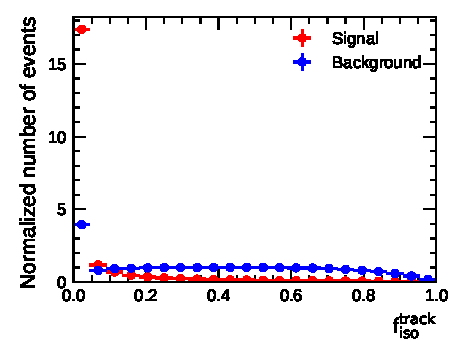
\includegraphics{./figures/baseline_bdt_vars/1p/SumPtTrkFrac.pdf}
    \subcaption{Momentum fraction of isolation tracks (1-prong).}
    \label{fig:sumpttrkfrac}
  \end{subfigure}\hfill
  \begin{subfigure}[t]{0.48\textwidth}
    \centering
    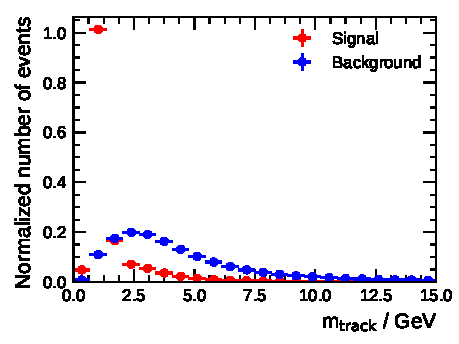
\includegraphics{./figures/baseline_bdt_vars/3p/massTrkSys.pdf}
    \subcaption{Mass of the track system (3-prong).}
    \label{fig:masstrksys}
  \end{subfigure}
  \caption{Examples of two important variables for discriminating hadronic tau
    decays from multijet events.}
  \label{fig:bdt_discriminants}
\end{figure}

\begin{table}[htb]
  \centering
  {\def\arraystretch{1.35}\small\begin{tabular}{ccc}
  \toprule
  Variable & 1-track & 3-track \\
  \midrule
  \smash{$f _\text{cent}$} & \textbullet & \textbullet \\
  \smash{$f_\text{leadtrack}^{-1}$} & \textbullet & \textbullet \\
  \smash{$R_\text{track}$} & \textbullet & \textbullet\\
  \smash{$\Delta R_\text{max}$} & & \textbullet \\
  \smash{$| S_\text{leadtrack} |$} & \textbullet & \\
  \smash{$S_\text{T}^\text{flight}$} & & \textbullet \\
  \bottomrule
\end{tabular}\hspace*{2em}
\begin{tabular}{ccc}
  \toprule
  Variable & 1-track & 3-track \\
  \midrule
  \smash{$f_\text{iso}^\text{track}$} & \textbullet & \\
  \smash{$f_\text{EM}^\text{track-HAD}$} & \textbullet & \textbullet \\
  \smash{$f_\text{track}^\text{EM}$} & \textbullet & \textbullet \\
  \smash{$p_\text{T}^\text{EM+track} / p_\text{T}$} & \textbullet & \textbullet \\
  \smash{$m_\text{EM+track}$} & \textbullet & \textbullet \\
  \smash{$m_\text{track}$} & & \textbullet \\
  \bottomrule
\end{tabular}

%%% Local Variables:
%%% mode: latex
%%% TeX-master: "../mythesis"
%%% End:
}
  \caption{Variables used for identification}
  \label{tab:baseline_variables}
\end{table}

Two important variables for the identification of hadronic tau lepton decays are
depicted in figure~\ref{fig:bdt_discriminants}. Figure~\ref{fig:sumpttrkfrac}
shows the momentum fraction of isolation
tracks~\smash{$f_\text{iso}^\text{track}$} indicating that that background
events reconstructed as 1-prong candidates often contain a large momentum
fraction. Moreover, the invariant mass of the track system for 3-prong
candidates in figure~\ref{fig:masstrksys} shows that the invariant mass for
signal events is peaked at below \SI{2.5}{\giga\electronvolt} while background
events can have large masses. Table~\ref{tab:baseline_variables} summarises
which variables are used in the different BDTs for 1- and 3-prong candidates.

\todo[inline]{Show 2D plot of signal \& background e.g. massTrkSys vs. EMPOverTrkSysP to
  motivate the use of MVA methods / BDTs}

\subsection{BDT-Setup}
The current implementation of the tau identification algorithm in the ATLAS
reconstruction framework uses BDTs trained with TMVA~\cite{tmva}. \todo{The
  config before the implementing the work in this thesis was:} The maximum depth
of individual decision trees is limited to~$d_\text{tree} = 8$ and the minimum
fraction of events contained in a node considered for further splitting
is~$f_\text{node}^\text{min} = \SI{0.1}{\percent}$. An ensemble
of~$N_\text{trees} = 100$ decision trees is trained using the \emph{AdaBoost}
algorithm with a learning rate $\beta = 0.2$, which determines the factor
multiplying the weight of incorrectly classified training examples (i.e.\ larger
learning rates increase this factor). The decision trees return estimated class
probabilities and no \emph{pruning} of statistically insignificant splits is
applied. This configuration is used as a starting point for further
optimisations. The full configuration of the TMVA-BDTs is summarised in
appendix~\ref{app:tmva_config} for reproducibility.

% \begin{align*}
%   N_\text{trees} &= 100 & d_\text{tree} &= 8 & \beta &= 0.2 \\
%   f_\text{node}^\text{min} &= \SI{0.1}{\percent} & N_\text{cuts} &= 200
% \end{align*}n
% as well as \texttt{UseYesNoLeaf} and no pruning.

\section{Event Simulation, Preselection and Reweighting}
\label{sec:bdt_eventsim}

\todo[inline]{$\sqrt{s} = \SI{13}{\tera\electronvolt}$, $\mu = \num{30}$}

For training and performance evaluation of the models simulated data is used.
The signal samples (i.e.\ hadronic tau lepton decays) are created by the process
$\gamma^* \rightarrow \tau \tau \, \text{(hadr.)}$, where at generator-level
leptonic decays are disabled. Moreover interference with and on-/ off-shell
production of the $\mathrm{Z}^0$ boson is disabled. The reason for not using a
sample employing the Drell--Yan process including interference and on- /
off-shell production of the $\mathrm{Z}^0$ boson is that the tau polarisation
changes for di-tau invariant masses close to the $\mathrm{Z}$-mass whereas
unpolarised taus are desired. Moreover the di-tau mass spectrum is smooth and
decreasing without increased statistics close to the $\mathrm{Z}$ mass which is
not needed for performance studies. The background for the identification
studies uses simulated dijet events with anti-$k_\text{T}$ truth jets (distance
parameter $R = 0.6$) with transverse momenta up
to~\SI{1800}{\giga\electronvolt}. A complete summary of the event samples can be
found in appendix~\ref{app:preprod_taus} and~\ref{app:preprod_dijets}. Both the
signal and the background samples are generated using \textsc{Pythia}~8 with the
A14 tune and leading order PDFs NNPDF23LO. \textsc{EvtGen} is used for b
fragmentation. The quark-gluon fraction is approximately \SI{60}{\percent}.

\begin{table}[htb]
  \centering
  {\small\begin{tabular}{lS[table-format=2.1]S[table-format=2.1]}
  \toprule
  & \multicolumn{2}{c}{Tau candidates / $10^6$} \\
  Sample & {1-prong} & {3-prong} \\
  \midrule
  Signal & 10.5 & 2.8 \\
  Background & 6.6 & 15.5 \\
  \bottomrule
\end{tabular}

%%% Local Variables:
%%% mode: latex
%%% TeX-master: "../mythesis"
%%% End:
}
  \caption{Number of candidates after baseline tau selection.}
  \label{tab:sample_size}
\end{table}

A preselection is applied to the event samples to match typical selections
applied at analysis level. Therefore the identification studies focus on
candidates with visible transverse
momenta~$p_\text{T} > \SI{20}{\giga\electronvolt}$. Reconstructed taus are
required to fall into the acceptance region of the tracking
system~$|\eta| < 2.5$ while rejecting candidates in the transition region
between barrel and end-cap of the calorimeter~$1.37 < |\eta| < 1.52$. The number
of reconstructed tracks (i.e.\ tracks classified as \emph{charged}) must be one
or three. Candidates in the signal samples are truth-matched to taus at
generator-level and the same selections (i.e.\ transverse momentum,
pseudorapidity, number of charged hadrons in the decay) are applied at
truth-level. The number of tau candidates after this baseline selection is
summarised in table~\ref{tab:sample_size}.

\begin{figure}[htb]
  \centering
  \begin{subfigure}[t]{0.48\textwidth}
    \centering
    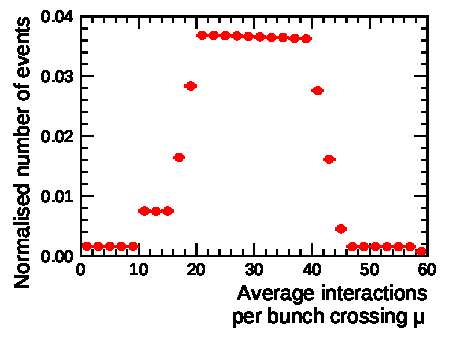
\includegraphics{./figures/bdt_perf/pt_mu_samples/mu.pdf}
    \subcaption{Average number of interactions per bunch crossing~$\mu$
      ($\langle \mu \rangle = 30$)}
  \end{subfigure}\hfill
  \begin{subfigure}[t]{0.48\textwidth}
    \centering
    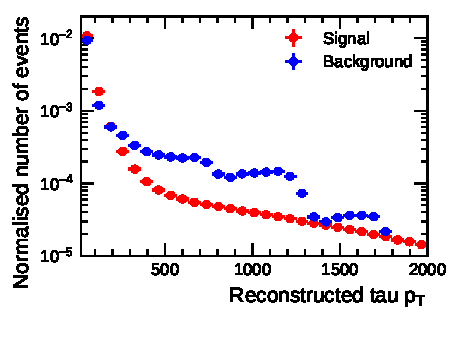
\includegraphics{./figures/bdt_perf/pt_mu_samples/pt.pdf}
    \subcaption{Transverse momentum spectrum of reconstructed tau candidates
      after baseline selection in $\gamma^* \rightarrow \tau \tau \, \text{(hadr.)}$
      and dijet samples with mass slices JZ1W to JZ6W.}
  \end{subfigure}
  \caption{Transverse momentum $p_\text{T}$ of tau candidates and pile-up
    spectrum of the samples.}
  \label{fig:pt_mu}
\end{figure}

In figure~\ref{fig:pt_mu} the distribution of reconstructed transverse
momenta~$p_\text{T}$ of tau candidates in the signal and background samples is
shown. Since the samples are created using different processes the
$p_\text{T}$-spectrum differ for both samples. When training the identification
algorithms distinguish signal and background by the momentum spectrum alone.
Therefore weights are applied to each tau candidates in the background sample
such that the weighted signal and background samples are indistinguishable in
the reconstructed transverse momentum.

% \todo[inline]{Reweighting, Quark-Gluon Fraction (3P: \SI{55}{\percent} excluding
%   bottom, \SI{58}{\percent} including bottom) (1P: \SI{55}{\percent} excluding
%   bottom, \SI{59}{\percent} including bottom); approx.\ \SI{60}{\percent}
%   quark-gluon fraction}

\section{Hyperparameter Optimisation}
\label{sec:bdt_hyperparam}

Machine learning algorithms have hyperparameters defining the complexity of the
model that cannot be determined as part of the training process. Often these
parameters need problem specific tuning to obtain the highest discriminative
power for a given algorithm. The BDTs of the 1- and 3-prong tau identification
are optimised separately with respect to the boosting algorithm used and the
most important hyperparameters.

Some input variables have highly skewed and long-tailed distributions leading to
suboptimal decision trees as TMVA uses equidistant sampling points for finding
the best possible split on a given variable. Therefore transformations are
applied to the input variables to improve . For this highly skewed distributions
are log-transformed while long-tailed distributions and outliers due to detector
resolution effects are clamped to fall into a specified range of values. The
exact transformations can be found in appendix~\ref{app:variable_transforms}.

Hold-out validation is used to measure how well the model generalises to data
that was not used to train the model. This is done by splitting the signal and
background samples into two equally sized samples called \emph{training} and
\emph{testing sample}. The \emph{training sample} is used to train the model and
the \emph{testing sample} is exclusively used to determine the performance
characteristics of the model. Unless otherwise noted, the metrics and figures
given in the following sections are evaluated on the \emph{testing sample}.

\subsection{Boosting Algorithm}
\label{sec:bdt_boosting}

In Chapter~\ref{sec:ml_boosting} two boosting algorithms \emph{AdaBoost} and
\emph{Gradient Boosting} were introduced. They are compared by training BDTs for
both algorithms and varying a boosting-specific parameter called the learning
rate. The learning rate for \emph{AdaBoost} is typically denoted by~$\beta$
while for the case of gradient boosting it is called \emph{shrinkage}~$\eta$.
Reducing the learning rate artificially slows down the boosting process by
causing additional trees to have a smaller impact on the ensemble.

The 1-prong tau identification BDTs with the input variables and configuration
summarised in Section~\ref{sec:bdt_tauid} are trained on tau candidates from the
signal and background samples (cf.\ Section~\ref{sec:bdt_eventsim}). The
learning rates for \emph{AdaBoost} and \emph{Gradient Boosting} are varied from
0.05 to 1.0 and the background rejection is calculated for a fixed signal
efficiency of \SI{60}{\percent}. For this a single cut on the output score of
the BDT is determined such that \SI{60}{\percent} of the tau candidates in the
signal sample pass this selection. This is an approximation to the \emph{tight}
working point of the tau-identification used in the ATLAS experiment.

\begin{figure}[htb]
  \begin{subfigure}[t]{0.48\textwidth}
    \centering
    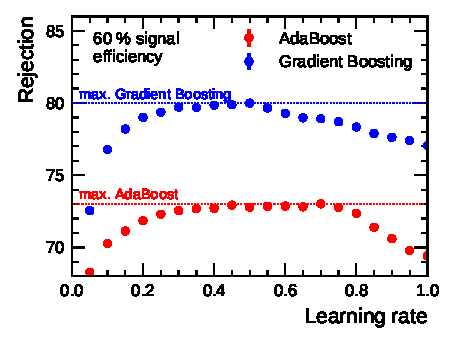
\includegraphics{./figures/bdt_perf/boosting.pdf}
    \subcaption{Rejection of 1-prong tau candidates from dijet events using BDTs
      trained with different boosting algorithms.}
    \label{fig:bdt_boosting_alg}
  \end{subfigure}\hfill
  \begin{subfigure}[t]{0.48\textwidth}
    \centering 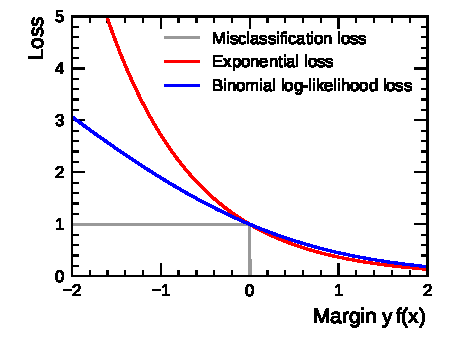
\includegraphics{./figures/theory/boosting_loss.pdf}
    \subcaption{Loss function of \emph{AdaBoost} (exp.\ loss), \emph{Gradient
        Boosting} (binom.\ log-likelihood loss) as a function of the
      margin~$y f(x)$ (true class $y \in \{-1, 1\}$, BDT score
      $f(x) \in [-1, 1]$).}
    \label{fig:boosting_loss}
    \todo[inline]{Margin from -1 to 1}
  \end{subfigure}
  \caption{Loss function investigation}
\end{figure}

In figure~\ref{fig:bdt_boosting_alg} the rejection is shown as a function of the
learning rate for both the \emph{AdaBoost} and \emph{Gradient Boosting}
algorithm. An improvement in rejection of approximately \SI{10}{\percent} is
observed when using \emph{Gradient Boosting}. The reason for this improvement is
the robust loss function used in the \emph{Gradient Boosting} implementation of
TMVA. The loss function (shown in figure~\ref{fig:boosting_loss}) puts less
weight on misclassified events ($y f(x) < 0$) such that it is more robust for
problems where signal and background are inseparable in certain regions of phase
space. For the tau identification algorithm this is often the case for jets
initiated by light quarks which more closely resemble hadronic decays of tau
leptons in the variables used for identification. Due to the significant
increase in rejection when using Gradient Boosting, it is used for the further
optimisation steps.

\subsection{Grid Search}
\label{sec:bdt_grid_search}
Aside from the boosting algorithm BDTs have important hyperparameters that need
to be optimised to obtain the best possible performance. These are the number of
trees~$N_\text{trees}$ in the ensemble and the learning rate~$\eta$, which are
boosting-specific parameters and are related as small learning rates require a
larger number of trees to converge. In addition the maximum tree
depth~$d_\text{tree}$ and the fraction of events required for node
splitting~$f_\text{node}^\text{min}$. Both parameters limit the depth of a tree
and therefore the allowed order of variable interactions in a single tree (e.g.\
$d_\text{tree} = 2$ allows interactions of up to two variables). Finally, bagged
boosting is investigated where each tree is grown using a random sample of
training events drawn with replacement from the full training sample. This
method aims to reduce overfitting (i.e.\ trees learning statistical fluctuations
in the training sample) and the corresponding hyperparameter is the fraction of
events~$f_\text{bag}$ in the random sample.

These hyperparameters are optimised by forming a grid in the parameter space and
training and evaluating a BDT trained for each point on this grid. The grid is
given by the following hyperparameter values
\begin{align*}
  N_\mathrm{trees} &\in \{25, 50, 100, 200, 400, 800\} & \eta &\in \{0.05, 0.1, 0.2, 0.4\} & d_\mathrm{tree} &\in \{4, 6, 8, 12, 16\}\\
  f_\mathrm{node}^\mathrm{min} &\in \{\SI{0.01}{\percent}, \SI{0.1}{\percent},\SI{1.0}{\percent}\} & f_\text{bag} &\in \{\text{None}, \SI{50}{\percent} \}
\end{align*}
resulting in a total of 720 grid points. The rejection is, analogously to the
previous section, calculated using a single cut on the output score to obtain a
signal efficiency comparable to the tight working points (i.e.\
\SI{60}{\percent} for 1-prong and \SI{45}{\percent} for 3-prong decays) used in
ATLAS.

\begin{figure}[htb]
  \begin{subfigure}[t]{0.48\textwidth}
    \centering
    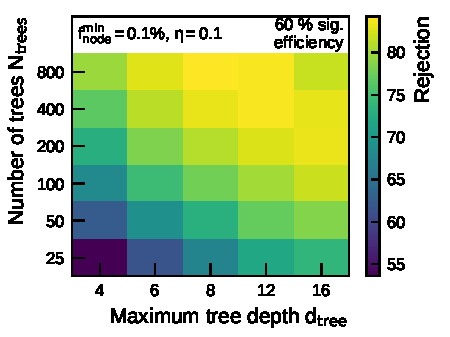
\includegraphics{./figures/bdt_perf/gridsearch_1p/scan_MaxDepth_NTrees.pdf}
    \vspace*{-1.6em}
    \subcaption{}
    \label{fig:gridscan_maxdepth_ntrees}
  \end{subfigure}\hfill
  \begin{subfigure}[t]{0.48\textwidth}
    \centering
    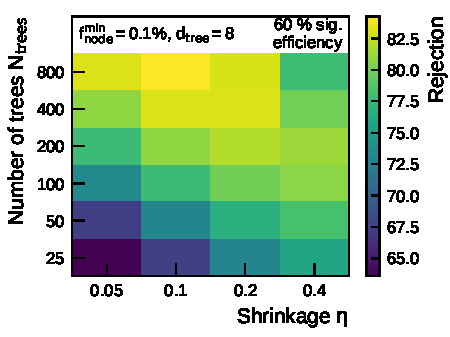
\includegraphics{./figures/bdt_perf/gridsearch_1p/scan_Shrinkage_NTrees.pdf}
    \vspace*{-1.6em}
    \subcaption{}
    \label{fig:gridscan_shrinkage_ntrees}
  \end{subfigure}
  \begin{subfigure}[t]{0.48\textwidth}
    \centering
    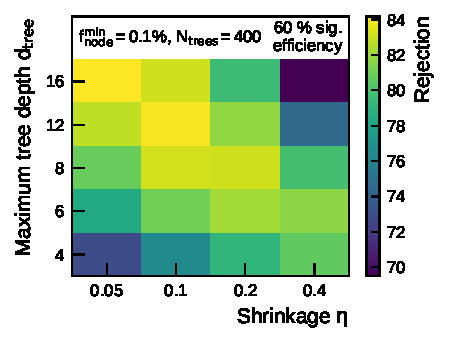
\includegraphics{./figures/bdt_perf/gridsearch_1p/scan_Shrinkage_MaxDepth.pdf}
    \vspace*{-1.6em}
    \subcaption{}
    \label{fig:gridscan_shrinkage_maxdepth}
  \end{subfigure}\hfill
  \begin{subfigure}[t]{0.48\textwidth}
    \centering
    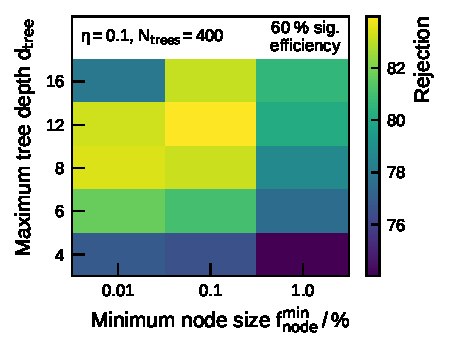
\includegraphics{./figures/bdt_perf/gridsearch_1p/scan_MinNodeSize_MaxDepth.pdf}
    \vspace*{-1.6em}
    \subcaption{}
    \label{fig:gridscan_minnodesize_maxdepth}
  \end{subfigure}
  \caption{Background rejection at \SI{60}{\percent} signal efficiency as a
    function of the BDT hyperparameters. Bagged boosting with a subsample
    fraction~$f_\text{bag} = \SI{50}{\percent}$ is used and the remaining
    parameters are fixed such that the 'best' BDT is contained within the
    plots.}
  \todo[inline]{Better word for 'best' as it is not the best BDT}
  \label{fig:hyperparameter_scan_1p}
\end{figure}

In Figure~\ref{fig:hyperparameter_scan_1p} the background rejection of the
1-prong tau-identification BDT is shown as a function of the hyperparameters of
the model. The relation between the hyperparameters and their impact on the
background rejection are discussed in the following.

The relationship of the number of trees~$N_\text{trees}$ in the ensemble with
the maximum tree depth~$d_\text{tree}$ and learning rate~$\eta$ of the gradient
boosting is shown in Figures~\ref{fig:gridscan_maxdepth_ntrees} and
\subref{fig:gridscan_shrinkage_ntrees}. A distinct trade-off can be observed
between the hyperparameters $d_\text{tree}$ and $N_\text{trees}$, where a large
number of shallow trees and a small number of deep trees can reach similar
background rejection. Moreover, small learning rates~$\eta$ require many trees
to properly fit the model. For a large number of trees and large maximum tree
depths or learning rates the model overfits, i.e.\ learns statistical
fluctuations in the training sample and therefore exhibits a decreased
generalisation performance. This effect can also be observed in
Figure~\ref{fig:gridscan_shrinkage_maxdepth}, where highly complex trees with a
depth of 16 can lead to overfitting if the learning rate is too large. The
importance of choosing an appropriate minimum node
size~$f_\text{min}^\text{node}$ is shown in
Figure~\ref{fig:gridscan_minnodesize_maxdepth}. If the minimum node size is
chosen too small the model does not properly fit the data. However, small
minimum node size can quickly lead to overfitting for decision trees with a
large maximum depth. The interplay of the maximum tree depth and minimum node
size when constraining \todo{continue}. The optimisation of the 3-prong
tau-identification shows similar results, which are summarised in
Appendix~\ref{app:grid_search_3p} and are omitted here for brevity.

\begin{table}[htb]
  \centering
  {\small\begin{tabular}{ll
  S[table-format=3.0]
  S[table-format=1.2]
  S[table-format=2.0]
  S[table-format=1.2]
  c}
  \toprule
  & Name & {$N_\text{trees}$} & {$\eta$} & {$d_\text{tree}$} & {$f_\text{node}^\text{min}$ / \si{\percent}} & {$f_\text{bag}$} \\
  \midrule
  \multirow{2}{*}{1-prong} & BDT A & 800 & 0.05 & 16 & 0.01 & -- \\
  & BDT B & 400 & 0.1 & 8 & 0.1 & \SI{50}{\percent} \\
  \midrule
  \multirow{2}{*}{3-prong} & BDT A & 800 & 0.1 & 16 & 0.01 & -- \\
  & BDT B & 800 & 0.4 & 6 & 0.1 & -- \\
  \bottomrule
\end{tabular}

%%% Local Variables:
%%% mode: latex
%%% TeX-master: "../mythesis"
%%% End:
}
  \caption{BDT configuration. Rejection is given at \SI{60}{\percent} for
    1-prong and \SI{45}{\percent} for 3-prong.}
  \label{tab:bdt_perfs}
\end{table}

\begin{figure}[htb]
  \begin{subfigure}[t]{0.48\textwidth}
    \centering
    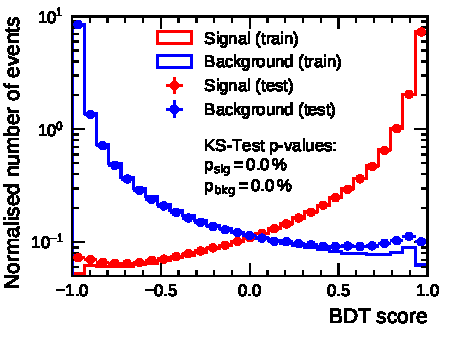
\includegraphics{./figures/bdt_perf/scores/grid_1p0304.pdf}
    \subcaption{Overtrained example 1-prong (BDT A):
      \mbox{$N_\text{Trees} = 800$},
      \mbox{$d_\text{Tree} = 16$},
      \mbox{$\nu = 0.05$, $f_\text{min.}^\text{Node} = \SI{0.01}{\percent}$},
      no bagging
    }
  \end{subfigure}\hfill
  \begin{subfigure}[t]{0.48\textwidth}
    \centering
    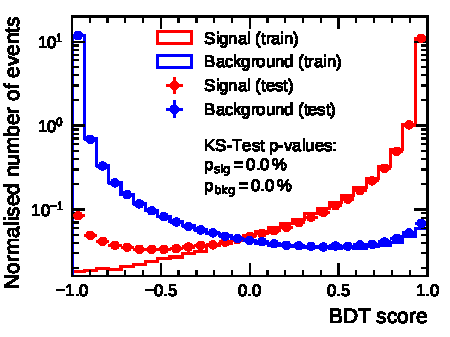
\includegraphics{./figures/bdt_perf/scores/grid_3p0317.pdf}
    \subcaption{Overtrained example 3-prong(BDT A):
      \mbox{$N_\text{Trees} = 800$},
      \mbox{$d_\text{Tree} = 16$},
      \mbox{$\nu = 0.1$, $f_\text{min.}^\text{Node} = \SI{0.01}{\percent}$},
      no bagging
    }
  \end{subfigure}
  \caption{'Overtraining' visible on the edges of the BDT score distribution
    (1-prong)}
  \label{fig:bdt_overfitting_scores}
\end{figure}

The grid search shows that the maximum of rejection is wide spanning over
multiple grid points. The configurations of the 1- and 3-prong BDTs are
summarised in Table~\ref{tab:bdt_perfs}. The models with the name \emph{BDT A}
consist of the BDT with the highest rejection at the corresponding signal
efficiency. One observes that these BDTs fall on an edge of the parameter grid,
indicating that a configuration with larger rejection can be found outside of
the scanned hyperparameter region. However, looking at the distribution of the
BDT scores for signal and background tau candidates on both the training and the
testing sample in Figure~\ref{fig:bdt_overfitting_scores} one observes that the
BDT score distributions deviate between training and testing sample. This
indicates that the BDTs are picking up statistical fluctuations in the training
samples and signals that these configurations are close to overfitting. The
deviations of the score distributions are most significant for the 1-prong
background and 3-prong signal distributions, due to the limited sample size
(cf.\ Table~\ref{tab:sample_size}).

% The one-prong BDT is optimised for efficiency of the tight working-point (in the
% scan no flattening was applied). However the 3-prong BDT was optimised for the
% loose working-point, because the rejection of the 3-prong ID is roughly one
% order of magnitude larger thus the tight working-point is not a stable metric
% considering the size of the available background sample.

\begin{figure}[ht]
  \begin{subfigure}[t]{0.48\textwidth}
    \centering
    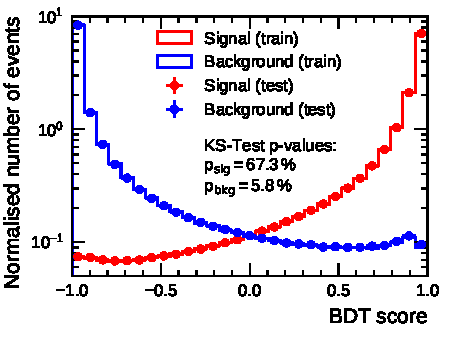
\includegraphics{./figures/bdt_perf/scores/grid_1p_subsampling0269.pdf}
    \subcaption{Good training (BDT B):
      \mbox{$N_\text{Trees} = 400$},
      \mbox{$d_\text{Tree} = 8$},
      \mbox{$\nu = 0.1$, $f_\text{min}^\text{Node} = \SI{0.1}{\percent}$},
      \mbox{$f_\text{bag} = \SI{50}{\percent}$}
    }
  \end{subfigure}\hfill
  \begin{subfigure}[t]{0.48\textwidth}
    \centering
    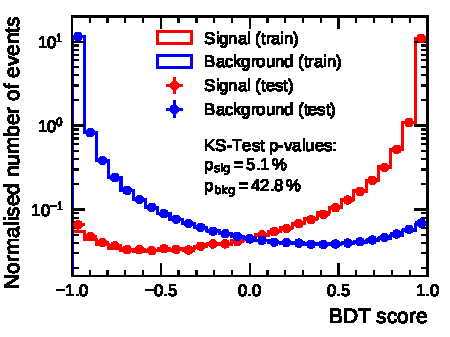
\includegraphics{./figures/bdt_perf/scores/grid_3p0327.pdf}
    \subcaption{Good training (BDT B):
      \mbox{$N_\text{Trees} = 800$},
      \mbox{$d_\text{Tree} = 6$},
      \mbox{$\nu = 0.4$, $f_\text{min}^\text{Node} = \SI{0.1}{\percent}$},
      \mbox{$f_\text{bag} = \text{None}$}
    }
  \end{subfigure}
  \caption{'Overtraining' visible on the edges of the BDT score distribution
    (1-prong)}
  \label{fig:bdt_ks5_scores}
  \todo[inline]{To appendix}
\end{figure}

Instead of choosing the BDT with the largest rejection, compatibility of the
signal and background BDT score distributions is required. This is done for
reasons of robustness to a potential decrease in training statistics for future
tunings. The compatibility of two distributions is measured using the $p$-value
of the Kolmogorov-Smirnov (KS) test. The configuration~\emph{BDT B} in
Table~\ref{tab:bdt_perfs} consists of the BDT with the highest rejection at the
specified signal efficiency, while also requiring that the $p$-value of the
KS-test between training and testing sample is larger than \SI{5}{\percent}. The
score distributions after requiring compatibility according to the KS-test is
shown in Figure~\ref{fig:bdt_ks5_scores}.

\begin{figure}[htb]
  \begin{subfigure}[t]{0.48\textwidth}
    \centering
    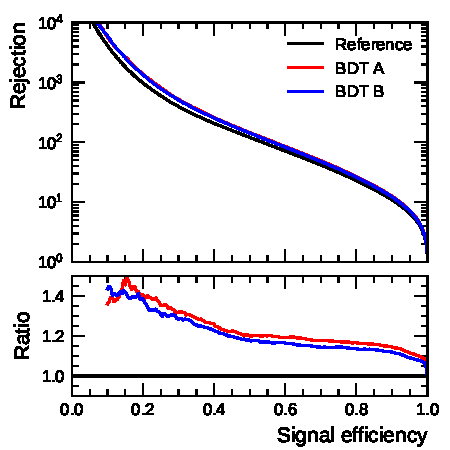
\includegraphics{./figures/bdt_perf/roc/bdt_1p_comparison.pdf}
    \subcaption{1-prong}
    \label{fig:bdt_1p_roc}
  \end{subfigure}\hfill
  \begin{subfigure}[t]{0.48\textwidth}
    \centering
    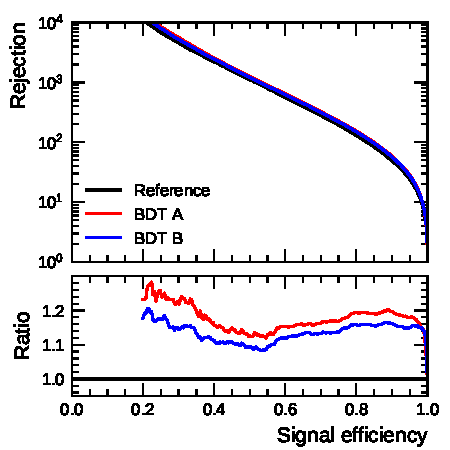
\includegraphics{./figures/bdt_perf/roc/bdt_3p_comparison.pdf}
    \subcaption{3-prong}
    \label{fig:bdt_3p_roc}
  \end{subfigure}
  \caption{\emph{ROC}-Curves. \mytodo{Rule of thumb? For 10 percent signal
      efficiency which factor of rejection do we get?}}
  \label{fig:bdt_rocs}
\end{figure}

The operating point of a BDT depends on the threshold applied to its output
score, thus defining a trade-off between signal efficiency and background
rejection. Figure~\ref{fig:bdt_rocs} shows the performance characteristics as
the classification threshold is varied and is also called the receiver operating
characteristic curve (ROC-curve). Comparing \emph{BDT A} and \emph{BDT B} for
the 1- and 3-prong identification, the decrease in rejection of the conservative
model is approximately \SI{5}{\percent} of the relevant efficiency ranges.
Moreover, the rejection of the conservative \emph{BDT B} improves on the
reference by \num{10} to \SI{16}{\percent} on the for tau-identification
relevant signal efficiency range. The rejection of the 3-prong BDT is
approximately one order of magnitude larger than for the 1-prong case. This can
largely be attributed to the availablility of invariant mass and secondary
vertex information.

\subsection{Working Points}
\label{sec:bdt_working_points}

\begin{table}[htb]
  \centering
  {\small\begin{tabular}{lcc}
  \toprule
  & \multicolumn{2}{c}{Signal efficiency} \\
  Working point & 1-prong & 3-prong \\
  \midrule
  Very Loose & 95\% & 95\% \\
  Loose & 85\% & 75\% \\
  Medium & 75\% & 60\% \\
  Tight & 60\% & 45\% \\
  \bottomrule
\end{tabular}

%%% Local Variables:
%%% mode: latex
%%% TeX-master: "../mythesis"
%%% End:
}
  \caption{Working point efficiencies}
  \label{tab:wp_eff}
\end{table}

\begin{figure}[ht]
  \begin{subfigure}[t]{0.48\textwidth}
    \centering
    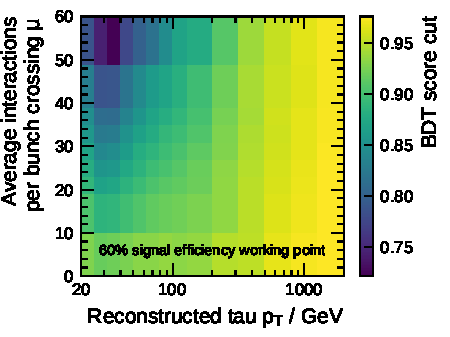
\includegraphics{./figures/bdt_perf/working_points/grid_1p_subsampling0269_wp.pdf}
    \subcaption{1-prong}
  \end{subfigure}\hfill
  \begin{subfigure}[t]{0.48\textwidth}
    \centering
    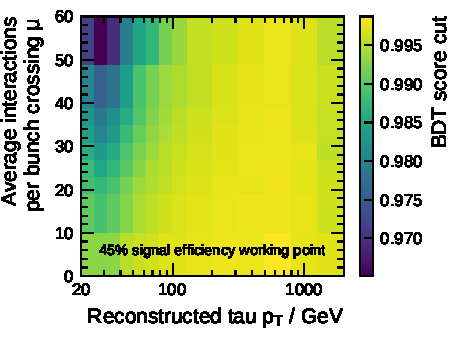
\includegraphics{./figures/bdt_perf/working_points/grid_3p0327_wp.pdf}
    \subcaption{3-prong}
  \end{subfigure}
  \caption{Working points (BDT A)}
\end{figure}

\begin{figure}[ht]
  \begin{subfigure}[t]{0.48\textwidth}
    \centering
    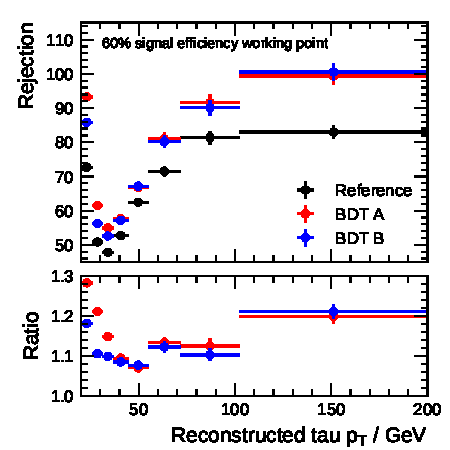
\includegraphics{./figures/bdt_perf/rejection/post_gridsearch_1p/rejection_tight.pdf}
    \subcaption{1-prong (tight)}
  \end{subfigure}\hfill
  \begin{subfigure}[t]{0.48\textwidth}
    \centering
    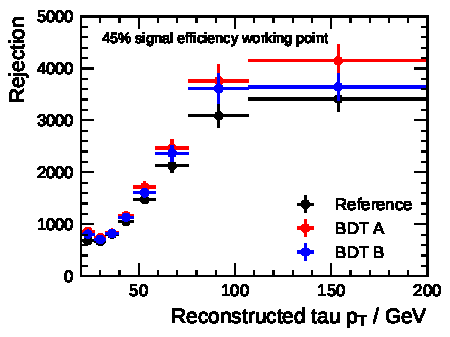
\includegraphics{./figures/bdt_perf/rejection/post_gridsearch_3p/rejection_tight.pdf}
    \subcaption{3-prong (tight)}
  \end{subfigure}
  \caption{Working points (BDT A) \mytodo{Larger pt range in appendix}.
    \mytodo{Ratio is bootstrapped due to highly correlated errors}}
  \todo[inline]{To appendix}
\end{figure}


\begin{itemize}
\item Working point: constant signal efficiency in different pt-regimes and
  pile-up environments. Rejection definitely not flat then!
\item Overall tighter cut for high $p_\text{T}$. Why?
\item Significant degradation at low $p_\text{T}$ for high pile-up. Why?
\item Overall slight improvement for lower pile-up scenarios. Why?
\item Show signal efficiency vs pt and mu
\end{itemize}

\section{Feature Selection}
\label{sec:bdt_feature_selection}
Before proceeding to feature selection a reliable hyperparameter setup has to be
found.
\subsection{Transverse Momentum Dependency of Features}
\label{sec:bdt_incl_pt}

\begin{figure}[ht]
  \begin{subfigure}[t]{0.48\textwidth}
    \centering
    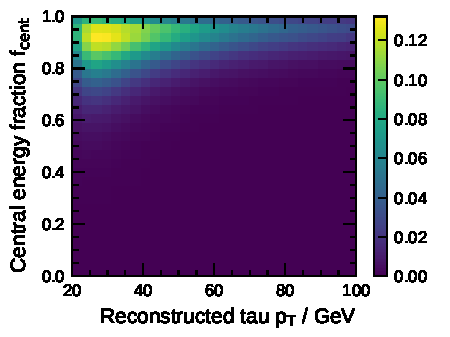
\includegraphics{./figures/bdt_perf/cent_frac_vs_pt_sig.pdf}
    \subcaption{Signal}
  \end{subfigure}\hfill
  \begin{subfigure}[t]{0.48\textwidth}
    \centering
    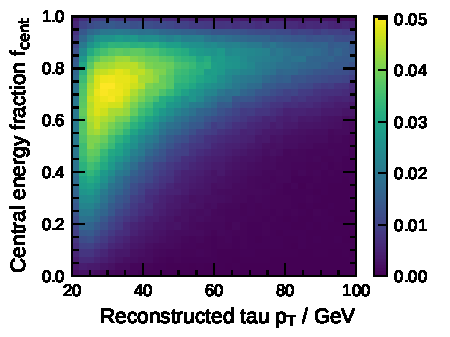
\includegraphics{./figures/bdt_perf/cent_frac_vs_pt_bkg.pdf}
    \subcaption{Background}
  \end{subfigure}
    \caption{$p_\text{T}$-dependency of the central energy fraction.}
  \label{fig:bdt_pt_dependency}
\end{figure}

A lot of the input features have (at least a small) dependency with the
reconstructed $p_\text{T}$ changing the separation of signal and background in
the features as a function of $p_\text{T}$. This effect has a large impact on
the overall isolation of the shower in the calorimeter and the tracks. An
example of this is the central energy fraction $f_\text{cent}$ shown in figure
\ref{fig:bdt_pt_dependency}. While the energy for signal events is mostly
contained in the cone of size $\Delta R < 0.1$ there are significant
contributions to the $0.1 < \Delta R < 0.2$ annulus for dijets reconstructed as
low $p_\text{T}$ tau candidates. To take advantage of the varying separation of
the input features in different $p_\text{T}$-regions the transverse momentum can
be included as an input to the BDT. It is important that the signal and
background samples used for training are reweighted such that no discrimination
purely based on the $p_\text{T}$-spectra of the samples is possible. For the use
of tau-identification in analyses the working point efficiencies in data must be
determined in a tag-and-probe measurement. For reconstructed taus with
transverse momenta greater than \SI{100}{\giga\electronvolt} there is limited
statistics. In practice the measured efficiencies need to be extrapolated to
higher $p_\text{T}$-regions and therefore it should be avoided to have an
explicit $p_\text{T}$-dependence in the BDT above this threshold (an implicit
dependency due to correlations of the regular features like the central energy
fraction can not be avoided). This is realised by \emph{clamping} the transverse
momentum
\begin{align*}
  p_\text{T}^\text{clamp} = \min(p_\text{T}, \SI{100}{\giga\electronvolt})
\end{align*}
and using this as an input to the BDT.

\begin{table}[htb]
  \centering
  \begin{tabular}{
  l
  p{1.5cm}
  S[table-format=1.1(1)]
  S[table-format=1.1(1)]
  S[table-format=1.1(1)]
  }
  \toprule
  & \multirow{2}{*}[-0.15em]{Variable} & \multicolumn{3}{c}{relative rejection gain / \si{\percent}} \\
  \cmidrule{3-5}
  & & {tight} & {medium} & {loose}\\
  \midrule
  \multirow{2}{*}{\vspace*{-0.2em}1-prong} & $p_\text{T}$ & 4.3 +- 0.4 & 4.4 +- 0.3 & 5.6 +- 0.2 \\[0.2em]
  & $p_\text{T}^\text{clamp}$ & 3.5 +- 0.3 & 3.8 +- 0.3 & 4.9 +- 0.2 \\
  \midrule
  \multirow{3}{*}{\vspace*{-0.4em}3-prong} & $p_\text{T}$ & 2.7 +- 0.9 & 3.9 +- 0.6 & 3.1 +- 0.3 \\[0.2em]
  & $p_\text{T}^\text{clamp}$ & 2.3 +- 0.9 & 3.6 +- 0.5 & 3.1 +- 0.3 \\[0.2em]
  & $f_\text{iso}^\text{track}$ & 3.0 +- 1.0 & 5.6 +- 0.6 & 6.6 +- 0.5 \\
  \bottomrule
\end{tabular}

%%% Local Variables:
%%% mode: latex
%%% TeX-master: "../mythesis"
%%% End:

  \caption{New variables}
  \label{tab:bdt_new_variables}
\end{table}

\subsection{Variable Importance}
\label{sec:bdt_var_importance}

\todo[inline]{Recursive Feature Elimination (also TMVA ranking?); Input variable
  correlations;}

\begin{figure}[ht]
  \begin{subfigure}[t]{0.33\textwidth}
    \centering
    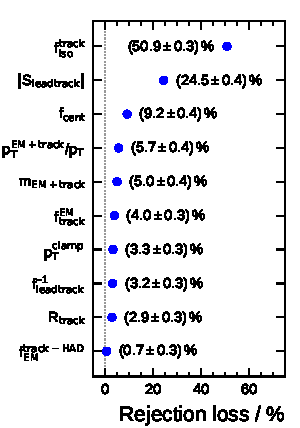
\includegraphics{./figures/bdt_perf/var_importance/1p_iter1.pdf}
    \subcaption{Iteration 1 (1-prong)}
  \end{subfigure}
  \begin{subfigure}[t]{0.33\textwidth}
    \centering
    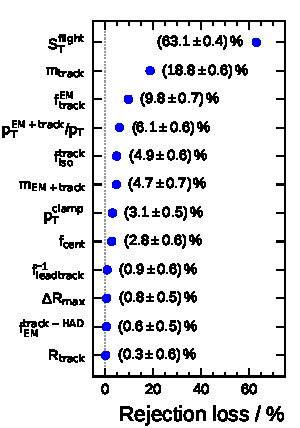
\includegraphics{./figures/bdt_perf/var_importance/3p_iter1.pdf}
    \subcaption{Iteration 1 (3-prong)}
  \end{subfigure}
  \caption{Variable importance. Averaged rejection loss over a gamma-tautau like
    dijet spectrum}
  \label{fig:variable_importance}
\end{figure}

One prong: Drop only ChPiEMEOverCaloEME \SI{0.7 +- 0.3}{\percent}

Three prong: Drop innerTrkAvgDist \SI{0.3 +- 0.6}{\percent}, then
ChPiEMEOverCaloEME \SI{1.2 +- 0.6}{\percent}, then etOverPtLeadTrk (do not drop)

Variable correlations, importance (dropped variables) \& dependence with
$p_\mathrm{T}$ (2D Hist - including pt), Variable Transformations (instead
of cutting out outliers), Partial Dependence, Including $p_\mathrm{T}$

\section{Identification Performance on Simulated Data}
\label{sec:bdt_perf}

\subsection{Performance in Simulation}
\label{sec:bdt_perf_sim}

\begin{figure}[ht]
  \begin{subfigure}[t]{0.48\textwidth}
    \centering
    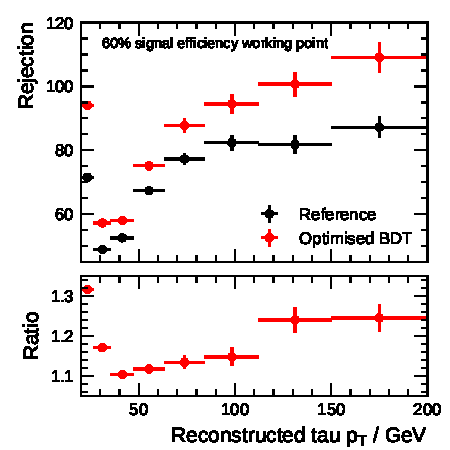
\includegraphics{./figures/bdt_perf/post_optimisation/rejection_tight_1p.pdf}
    \subcaption{1-prong. (Dropped ChPiEMEOverCaloEME)}
  \end{subfigure}\hfill
  \begin{subfigure}[t]{0.48\textwidth}
    \centering
    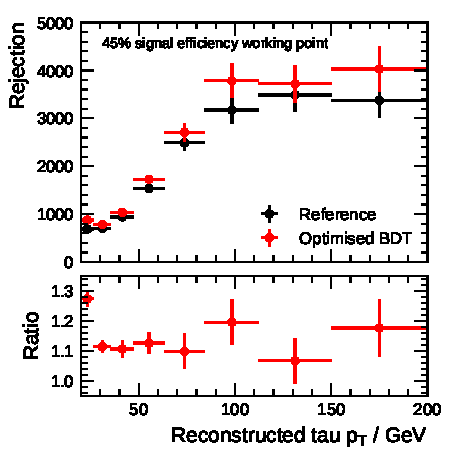
\includegraphics{./figures/bdt_perf/post_optimisation/rejection_tight_3p.pdf}
    \subcaption{3-prong. (Dropped innerTrkAvgDist and ChPiEMEOverCaloEME)}
  \end{subfigure}
  \caption{Working points}
\end{figure}



\todo[inline]{Moneyplot: Rejection vs pt for tight working points after all
  improvements vs.\ old setup }

Impact on (reconstructed) decay modes (?)

\todo[inline]{Partial Dependence Plots}

\todo[inline]{Give explanation for how the rejection vs pt plot looks}

\subsubsection{Performance on Quark- / Gluon-initiated Jets}
\label{sec:bdt_perf_quark_gluon}

Impact of Quark / Gluon initiated jets on Tau-ID (i.e. performance of ID
on Quark / Gluon jets)

\todo[inline]{Quark/Gluon performance}

\subsection{Performance on Data}
\label{sec:bdt_perf_data}

\todo[inline]{Performance on TAUP4?}

%%% Local Variables:
%%% mode: latex
%%% TeX-master: "mythesis"
%%% End:
